\chapter{Resultados} \label{cap6}
\addcontentsline{toc}{chapter}{Resultados}

\begin{flushright}
\begin{minipage}{7.85cm}
    {\em Si buscas resultados distintos, no hagas siempre lo mismo.} \\ Albert
    Einstein
\end{minipage}
\end{flushright}

\vspace*{5mm}

\section{Preparando el Escenario}

Para poder validar el trabajo realizado, hemos de simular lo ocurrido en el
caso guía y comparar los resultados con lo que realmente pasó. Para ello hemos
recopilado información de la inundación provocada por el paso del huracán
Katrina por Nueva Orleans en el año 2005.

Utilizando la información obtenida, creamos un escenario de simulación que
recrea la catástrofe que asoló la ciudad de Nueva Orleans. Como datos de
entrada utilizamos las roturas de los diques que contenían al río Mississippi
-nuestras Entradas de Agua-, la distribución de la población -los agentes
Peatón-, el terreno real y las calles reales de la ciudad.

\subsection{Área de simulación}

El huracán Katrina afectó a una parte considerable del estado de Luisiana, pero
nosotros nos centraremos en la ciudad de Nueva Orleans. En concreto el área que
se inundó de la ciudad viene resaltada en la siguiente imagen.

\begin{figure}[H]
 \centering
 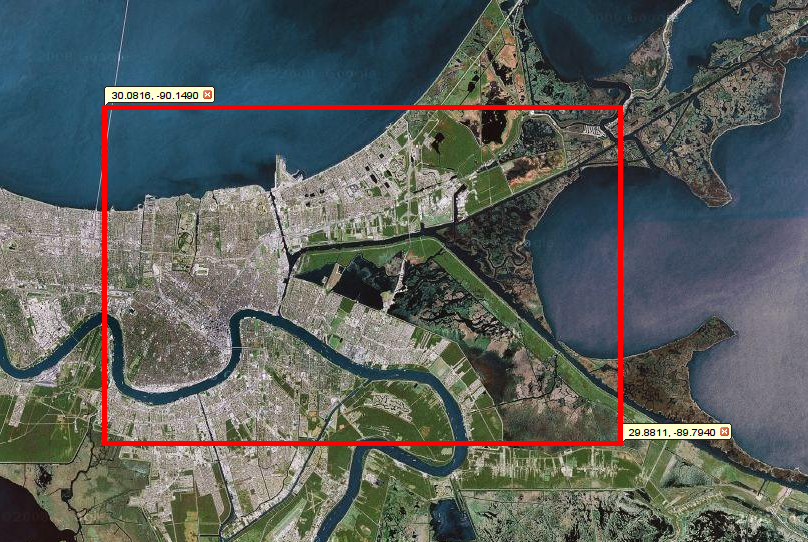
\includegraphics[height=120mm,angle=90]{figuras/cap6/NOarea1.png}
 \caption{Área de simulación}
\end{figure}

Al producirse la inundación por el desbordamiento del río, entre el mismo río y
los canales que atraviesan la ciudad dividieron la inundación en tres grandes
zonas casi independientes\cite{Pennington06}. En la siguiente imagen se puede
apreciar la división de la inundación en las tres zonas afectadas.

\begin{figure}[H]
 \centering
 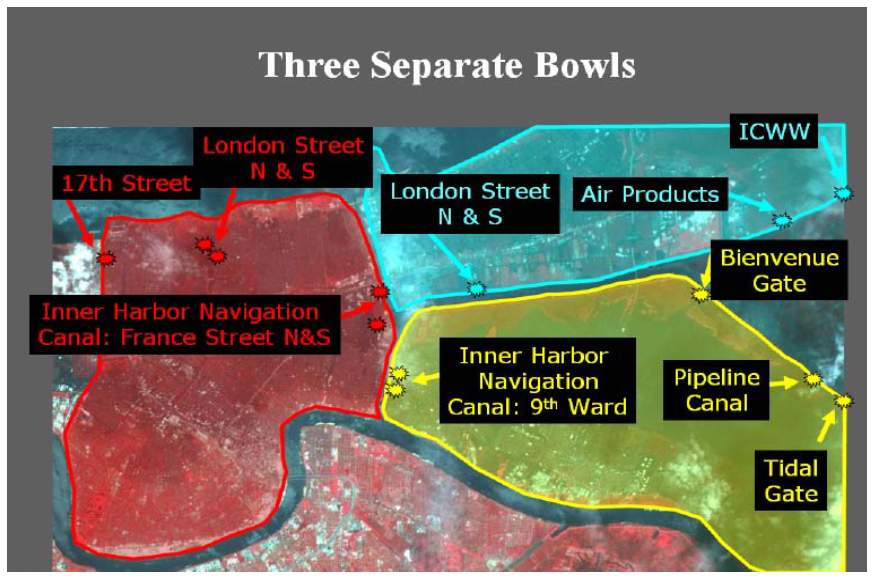
\includegraphics[width=100mm]{figuras/cap6/affected.png}
 \caption{División en 3 zonas del área afectada}
\end{figure}

Al ser el mismo río el que separa las diferentes zonas, éstas pueden simularse
por separado. Para ahorrar recursos y reducir la carga computacional nos
planteamos la creación de tres escenarios de simulación separados. Las
siguientes imágenes muestran las áreas de cada uno de dichos escenarios.

\begin{figure}[H]
 \centering
 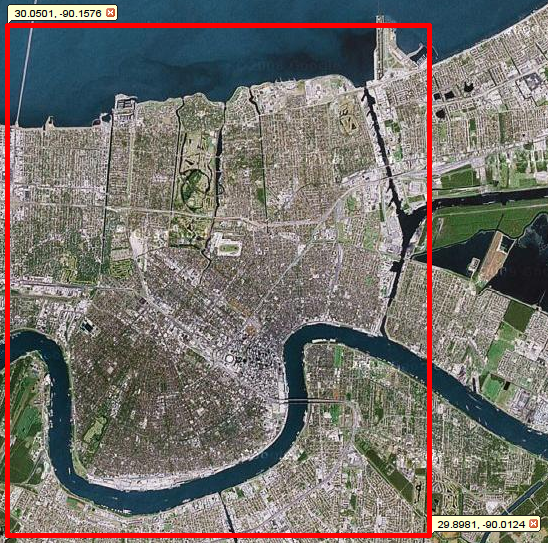
\includegraphics[width=120mm]{figuras/cap6/NOarea2.png}
 \caption{Zona 1 de simulación}
\end{figure}

\begin{figure}[H]
 \centering
 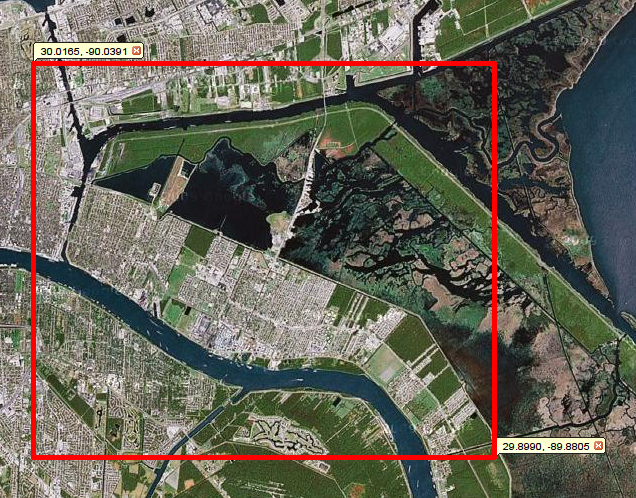
\includegraphics[width=135mm]{figuras/cap6/NOarea3.png}
 \caption{Zona 2 de simulación}
\end{figure}

\begin{figure}[H]
 \centering
 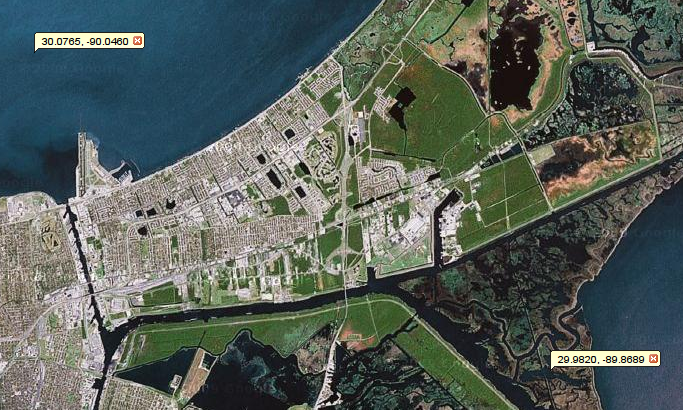
\includegraphics[width=135mm]{figuras/cap6/NOarea4.png}
 \caption{Zona 3 de simulación}
\end{figure}

\subsection{Elevación del Terreno}

Para poder simular la inundación uno de los datos que tenemos que obtener es
la elevación del terreno. Para una zona tan grande como Nueva Orleans hacen
falta millones de datos de altura, sin embargo para nuestra simulación nos hemos
limitado a la parte de Nueva Orleans que resultó mas afectada, y hemos utilizado
hexágonos de 50 metros de tamaño.

Dado que el servicio web del que obtenemos la información nos obliga a
solicitar las alturas de las casillas una a una, y a que son muchísimas
casillas, la obtención de estos datos ha sido muy lenta. Es en estos casos
cuando la \hyperref[cache]{caché de alturas} demuestra su utilidad, dado que
nos permite ejecutar varias simulaciones sin tener que volver a descargar las
alturas.

\subsection{Roturas de los Diques}

La causa de que la ciudad se inundase fue que los diques no resistieron el paso
del huracán, se rompieron en múltiples localizaciones y el crecido Mississippi
anegó los barrios de la ciudad. Las posiciones\cite{Pennington06} de estas
roturas son las entradas de agua a la simulación.

\begin{figure}[H]
 \centering
 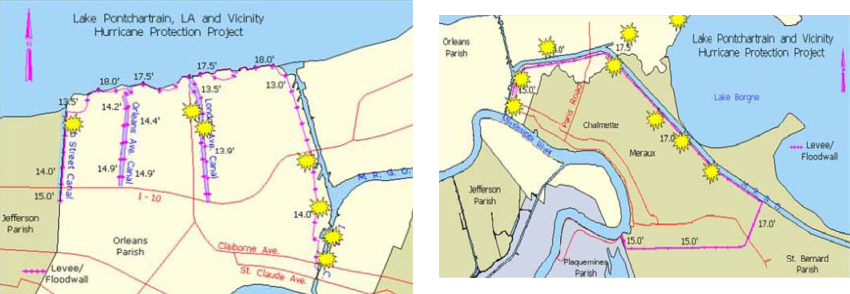
\includegraphics[width=135mm]{figuras/cap6/dikes.png}
 \caption{Localización de las roturas de los diques}
\end{figure}

En las siguientes imágenes se muestran geolocalizadas las posiciones de las
diferentes roturas que sufrieron los diques. En cada una de estas coordenadas
estará posicionado en la simulación un agente {\bf Entrada de Agua}.

\begin{figure}[H]
 \centering
 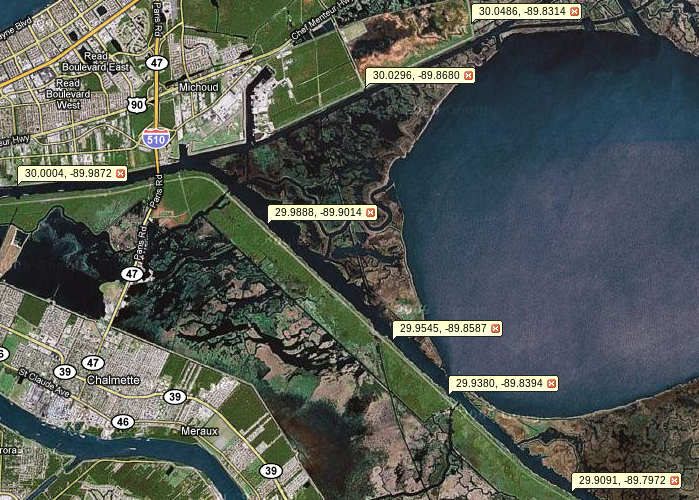
\includegraphics[width=135mm]{figuras/cap6/dikes1.png}
 \caption{Detalle de las roturas de los diques 1}
\end{figure}

\begin{figure}[H]
 \centering
 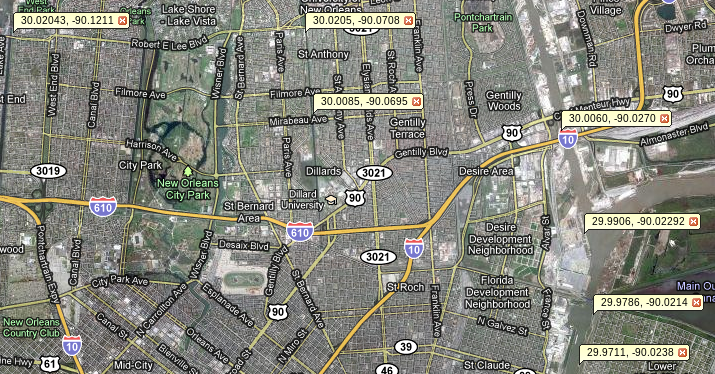
\includegraphics[width=135mm]{figuras/cap6/dikes2.png}
 \caption{Detalle de las roturas de los diques 2}
\end{figure}

\subsection{Refugios y Rutas de Evacuación}

En un principio se utilizó el {\em Louisiana Superdome} -una gran instalación
deportiva y de exhibición ubicada en el distrito central de negocios de Nueva
Orleans- como refugio, pero pasados unos días fue evacuado también. Dicha
instalación en encuentra en las coordenadas geográficas 29.950931°, -90.081364°.

Aparte del {\em Superdome}, no hubo otros refugios notables, si no que lo que se
hizo fue una evacuación completa de la ciudad. Por ello, hemos marcado como
objetivos tres posibles rutas de escape para los ciudadanos.

También consideramos que los edificios de los cuales podemos obtener
información a través de OSM pudieron ser refugios de emergencia donde
temporalmente pudieron refugiarse algunos ciudadanos. % TODO quitar?

\begin{figure}[H]
 \centering
 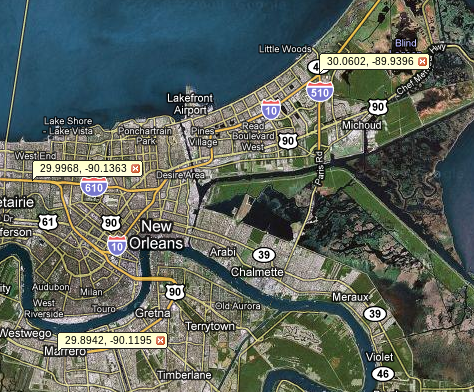
\includegraphics[width=105mm]{figuras/cap6/evacuation.png}
 \caption{Posibles rutas de evacuación y posición del Superdome}
\end{figure}

\section{Resultados}

A la hora de simular un escenario tan inmenso nos hemos encontrado con
numerosos problemas, el enorme tamaño del área de simulación nos ha obligado a
buscar máquinas potentes con las que hacer la simulación.

Nuestros tutores nos brindaron la posibilidad de utilizar una máquina del
departamento, que cuenta con ocho núcleos de procesamiento. Por desgracia, no
tiene suficiente memoria como para manejar todos los datos, como descubrimos
amargamente al tratar de simular en dicha máquina.

Sacrificando la velocidad de procesado y en busca de mayor cantidad de memoria
migramos a otra máquina. La simulación se realizó en ordenador con las
siguientes características:

\begin{itemize}
 \item Dos núcleos de procesado a % TODO
 \item Cuatro gigas de memoria RAM
% TODO
\end{itemize}

\subsection{Escenario Simulado}

\lstinputlisting[caption=Escenario post Katrina
simulado]{capitulo6/Katrina.scen}

Como hora inicial hemos tomado las 9:00 AM del día 29 de Agosto de 2005, pues
fue cuando se produjo la primera rotura de uno de los diques de
contención\cite{DeLozier}.

% TODO

\subsection{Visualización de Resultados}
%Ventanitas del simulador o capturas de google earth
\section{Simulación frente Realidad}
%Es cuestion de preparar un escenario de nueva orleans y comparar con la
%bibliografia

En la siguiente imagen podemos observar qué zonas quedaron dañadas en Nueva
Orleans tras la inundación\cite{Gabe05}.

\begin{figure}[H]
 \centering
 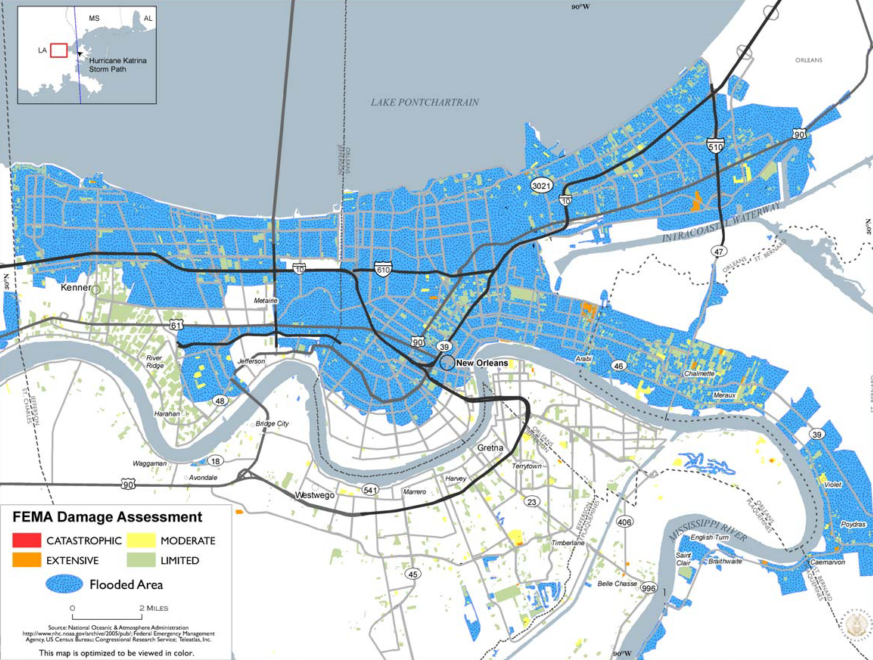
\includegraphics[width=135mm]{figuras/cap6/NOdamage.png}
 \caption{Daños reales en Nueva Orleans}
\end{figure}

%%% Local Variables:
%%% mode: latex
%%% TeX-master: "../dissim"
%%% End: